%%%%%%%%%%%%%%%%%%%%%%%%%%%%%%%%%%%%%%%%%%%%%%%%%%%%%%%%%%%%%%%%%%%%%%%%%%%%%%%%%%%%%%%%%%%%%
%%									Chapitre 1											%
%%%%%%%%%%%%%%%%%%%%%%%%%%%%%%%%%%%%%%%%%%%%%%%%%%%%%%%%%%%%%%%%%%%%%%%%%%%%%%%%%%%%%%%%%%%%%
\chapter{Illustration des principales commandes}
	\citationChap{
	The thing about quotes on the internet is that you can not confirm their validity
	}{Abraham Lincoln}
	\minitoc
	\newpage

%%%%%%%%%%%%%%%%%%%%%%%%%%%%%%%%%%%%%%%%%%%%%%%%%%%%%%%%%%%%%%%%%%%%%%%%%%%%%%%%%%%%%%%%%%%%%



% Début du chapitre

\section{Exemple minimal}
	\subsection{Glossaire et citations}
		On va raconter n'importe quoi à propos des \gls{asb}, juste pour illustrer à quoi ressemblent les différents glossaires. On pourrait tout aussi bien converser sur la pertinence de l'utilisation des \gls{csl} pour caractériser les \glspl{macle} du \gls{rutile}. Et pour craner un peu, je vais citer le merveilleux travail de \citet{depriester2014thermomechanical}. Maintenant que les \gls{asb} et \gls{csl} ont été définies, plus besoin de détailler leurs significations.
		
	\subsection{Tableaux et figures}
	On va ici placer des éléments graphiques (voir tableau~\ref{tab:exemple} et figure~\ref{fig:exemple}), juste pour avoir des entrées dans les listes des figures et des tableaux. On remarquera l'utilisation des sous-figures~\ref{sub:Antibes} et~\ref{sub:SaintJeannet}.
	
	\begin{tableth}
		\caption[Légende courte pour l'exemple de tableau]{Un tableau avec une légende tellement longue que ce serait hideux dans la liste des tableaux}
			\label{tab:exemple}
		\begin{tabular}{c|c}
			Coucou	& Au revoir\\
			\hline
			maman	& papa
		\end{tabular}
	\end{tableth}

	\begin{figureth}
		\begin{subfigureth}{0.4\textwidth}
			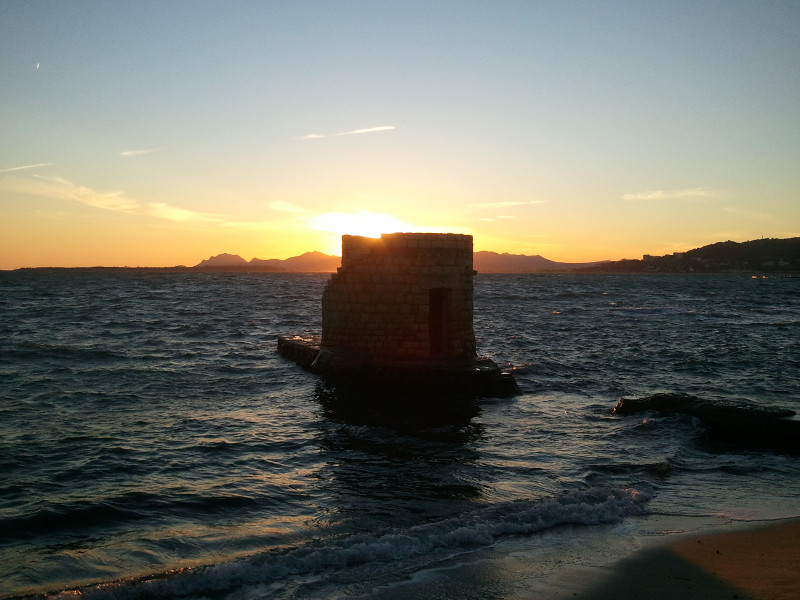
\includegraphics[width=\linewidth]{Antibes}
			\caption{Photo du Cap d'Antibes}
				\label{sub:Antibes}
		\end{subfigureth}
		\begin{subfigureth}{0.4\textwidth}
			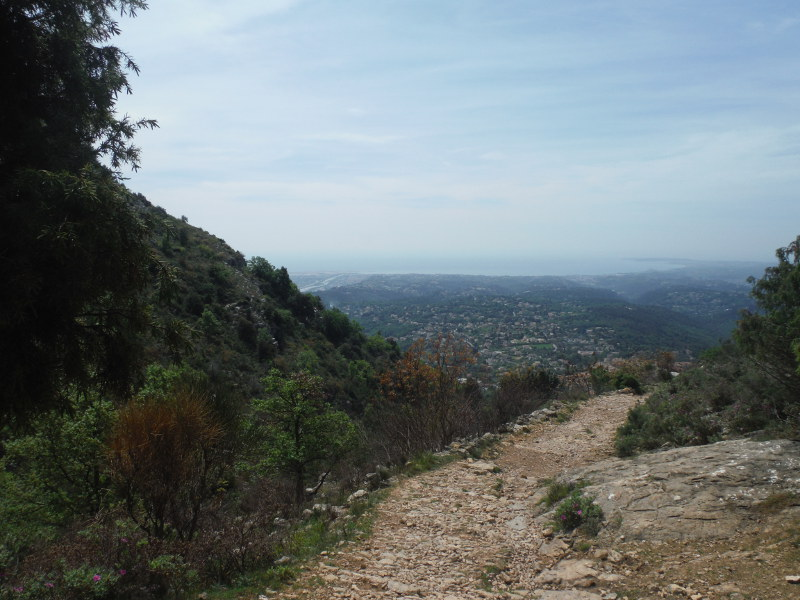
\includegraphics[width=\linewidth]{SaintJeannet}
			\caption{Saint Jeannet, depuis son Baou}
				\label{sub:SaintJeannet}
		\end{subfigureth}
		\caption[Légende courte pour la figure]{Exemple d'utilisation des sous-figures. J'utilise ici volontairement une légende longue.}		
			\label{fig:exemple}
	\end{figureth}
	
	\subsection{Symboles mathématiques}
	Rien de spécial à propos des math, hormis l'illustration des symboles listés en fin de document, tels \gls{alpha} ou \gls{gamma}, qui peuvent être utilisés indifféremment en mode \emph{in-line} ou dans des équations\footnote{Le lecteur notera que \texttt{hyperref} ajoute un lien cliquable sur chaque entrée des différents glossaires.} :
	\begin{equation}
		\gls{alpha}=\nicefrac{\gls{gamma}}{2}
		\label{eq:alphagamma}
	\end{equation}
Les entrées des glossaires peuvent même être appelés dans des figures (PDF avec surcouche \LaTeX, ou Ti\textit{k}Z).
	

\section{Deuxième paragraphe}
\blindtext

\bibliographystyle{francaissc}
\bibliography{Chapitre1/Biblio}